\subsection{Top Searches and Trend} \label{viztopsearches}
We used tree map visualization to plot the top search strings for every
individual years. The tree maps for individual years, specifically 3 years
before the website was reorganized and 1 year after the website was
reorganized are placed side by side. This helps in understanding the trend of
 the search strings. Figure \ref{fig:topsearches} provides the screenshot of
 the visualization. Please refer to the Tableau live implementation to see
 the interactive version of this visualization which showcases many details
 on the mouse-over.

The analysis of this visualization clearly identifies the trend. Before 2016,
 the maximum search strings were related to 'periodic table of elements'
 while in 2016 the focus is shifted towards 'mapping science'. However, these
   two topics are consistently amongst the top 10 searches throughout the
   analysis period.

\begin{figure}
\centering
\fbox{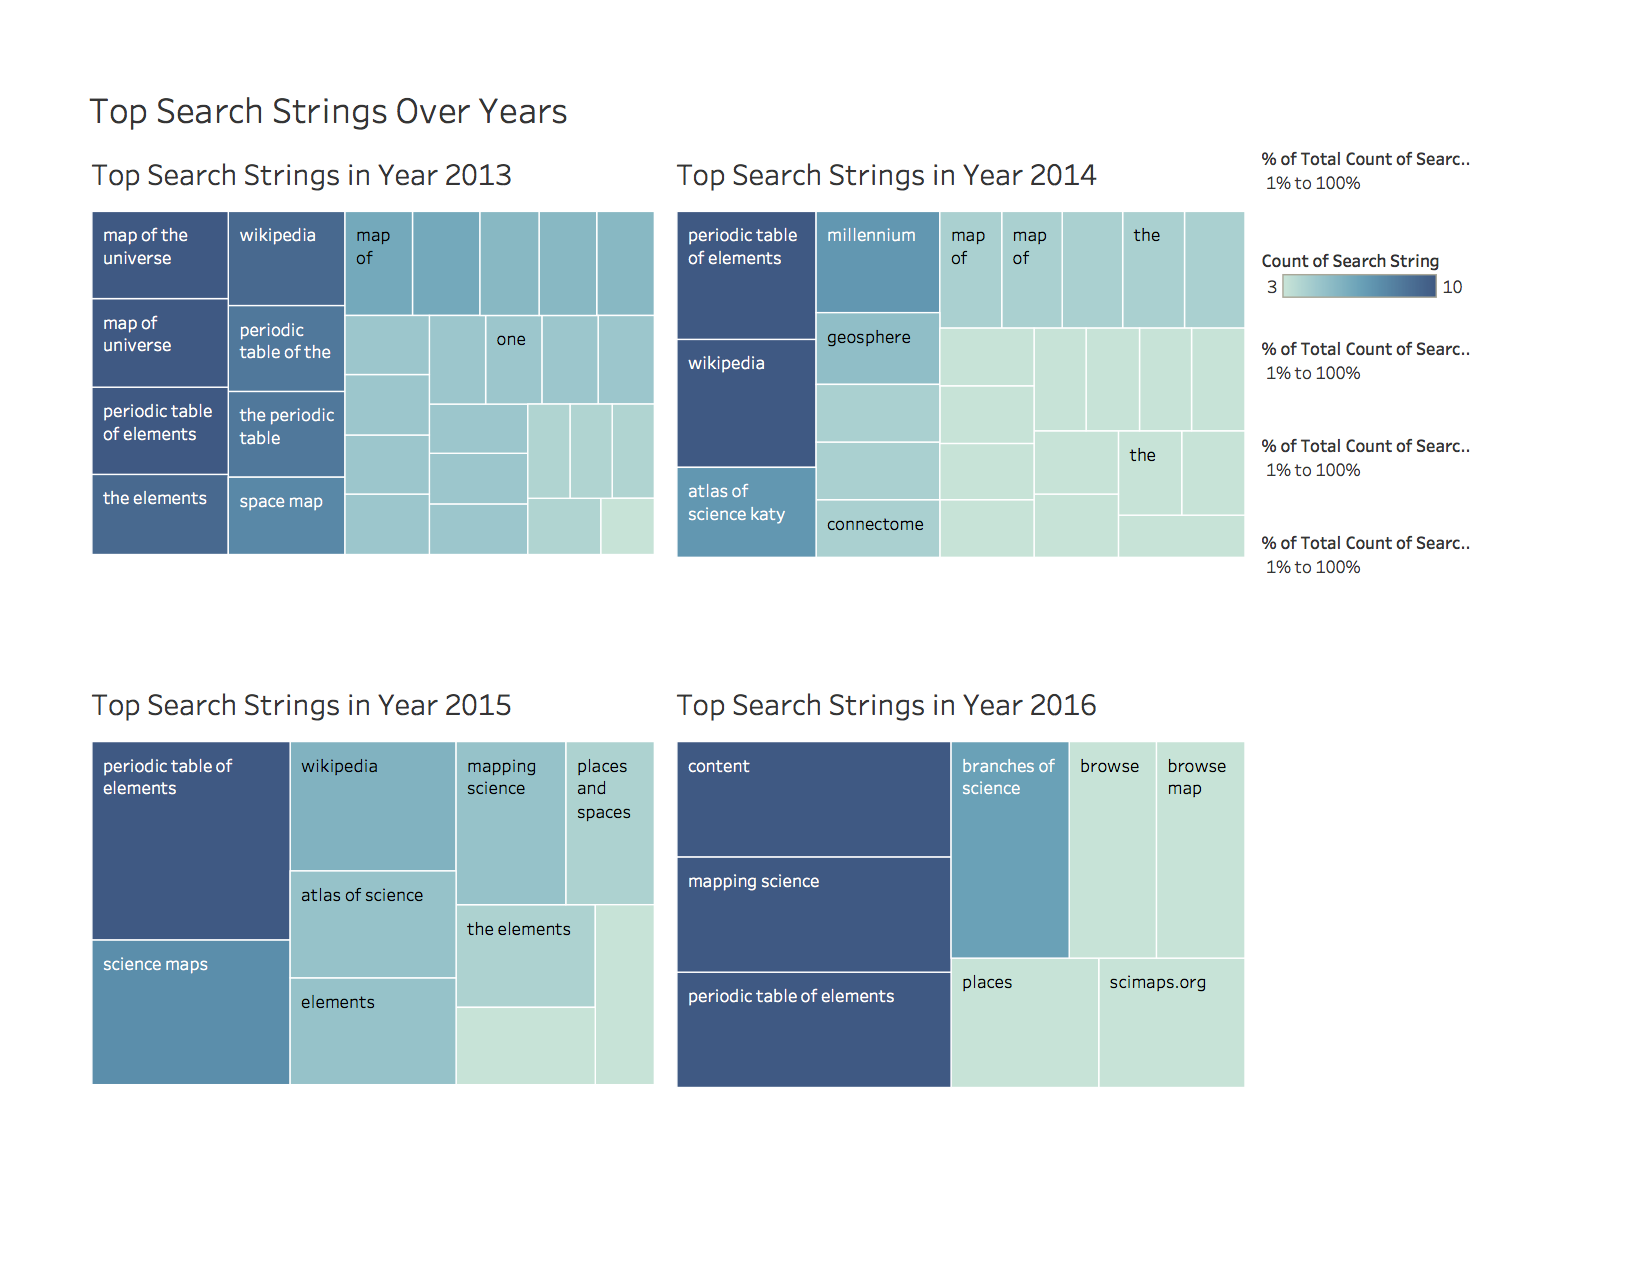
\includegraphics[width=\linewidth]{img/top_search_string_2013_to_2016.png}}
\caption{Top Search Strings in year 2013 to year 2016.}
\label{fig:topsearches}
\end{figure}
